\documentclass[12pt, aspectratio=43]{beamer}

\usepackage{pablo-beamer}

\begin{document}

\setcounter{section}{1}
\section{Multiplication d'un vecteur par un nombre réel}

\begin{frame}~

  \begin{center}
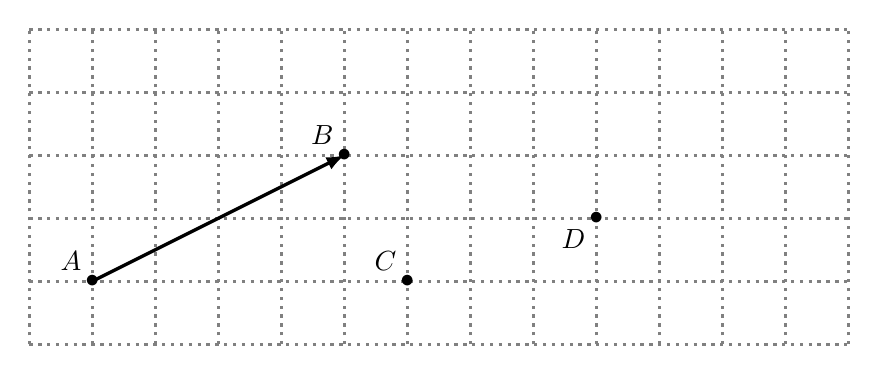
\begin{tikzpicture}[scale=0.8,very thick]
  \draw[dotted,color=gray,step=1] (0,0) grid (13,5);
  \draw[-latex] (1,1) -- (5,3);
  \draw (1,1) node{$\bullet$} node[above left]{$A$};
  \draw (5,3) node{$\bullet$} node[above left]{$B$};
  \draw (6,1) node{$\bullet$} node[above left]{$C$};
  \draw (9,2) node{$\bullet$} node[below left]{$D$};
\end{tikzpicture}
\end{center}

\begin{enumerate}
  \item Recopier le vecteur $\vecteur{AB}$ sur votre cahier.
  \item Placer le point $C$ tel que $\vecteur{CE}=2\vecteur{AB}$.
  \item Compléter : $\vecteur{AB}=\ldots\vecteur{CE}$.
  \item Placer le point $F$ tel que $\vecteur{DF}=\frac{1}{3}\vecteur{AB}$.
  \item Placer le point $G$ tel que $\vecteur{BG}=\vecteur{AB}+\vecteur{BA}$.
  \item Compléter : $\vecteur{AB}=\ldots\vecteur{BA}$.
\end{enumerate}
\end{frame}

\end{document}
